\documentclass{beamer}

\usepackage{svg}

\usetheme{Boadilla}

% Title
\title{Why Should You Care About Free Software}
\subtitle{Linux Week \the\year{}}
\author{Soham S Gumaste}
\date{\today}
\institute{Linux Users Group @ UIC}

\begin{document}
\begin{frame}
	\titlepage
\end{frame}

\begin{frame}{Table of Contents}
	\tableofcontents[pausesections]
\end{frame}

\section{What is Free Software}
\begin{frame}{The Four Freedoms}
	\textbf{Free Software} is any software that guarantees the following to
	its users:
	\pause
	\begin{enumerate}
		\item Freedom to run the program however you want.
			\pause
		\item Freedom to study how the program works and change it to
			do what you want.
			\pause
		\item Freedom to redistribute to others in need.
			\pause
		\item Freedom to distribute modified copies for others to
			benefit.
	\end{enumerate}
\end{frame}

\begin{frame}{Implications}
	These freedoms also imply the following:
	\pause
	\begin{enumerate}
		\item Freedom to NOT run the software! (Is everything on your
			computer running with your consent?)
			\pause
		\item Freedom to delete the software from your computer. (Try
			deleting Cortana from Windows!)
			\pause
		\item Access to the source code of the program \textbf{AND}
			documentation without excessive copyright restrictions.
	\end{enumerate}
\end{frame}

\begin{frame}{Free as in FREEDOM}
	\begin{block}{}
		{\large ``Free as in freedom, not as in free speech.''}
		\vskip5mm
		\hspace*\fill{\small--- Richard Stallman}
	\end{block}

	\pause

	The \underline{free} in freedom does NOT refer to money! Free Software
	is about computer user's \textbf{rights} not \textbf{wallets}, although
	the latter is \textbf{beneficial} too.
\end{frame}

\begin{frame}{Think about Microsoft Word}
	\pause
	\begin{itemize}
		\item Can you study the code?
			\pause
		\item Can you learn what it is doing on your computer?
			\pause
		\item What is stopping Word from running something you don't
			want? (Spoiler alert: They already do!)
			\pause
		\item Can you change it to do what you want?
			\pause
	\end{itemize}

	Even if Microsoft Word was free of charge, it would NOT affect any of
	the above questions.
\end{frame}

\begin{frame}{Do you own your computer?}
	Non-Free software stops \textbf{you} from doing what you want with
	\textbf{your} computer.
	
	\pause
	\begin{itemize}
		\item Windows does not allow you to (easily) remove the junk
			from the start menu.
			\pause
		\item Adobe software has \textbf{mandatory} updates, some of
			which have even removed access to COLORS! (Look up
			Adobe Pantone Colors)
			\pause
		\item Apple Computers only run software blessed (signed) by
			Apple (Developer Certificates, App Keys)
			\pause
	\end{itemize}

	Do you \textbf{really} own your computer?
\end{frame}

\section{Benefits of Free Software}
\begin{frame}{Table of Contents}
	\tableofcontents[currentsection]
\end{frame}

\begin{frame}{Complete User Freedom}
	With Free Software, users have total control over the software they are
	running, instead of software developers dictating what users can or
	cannot do.

	\pause

	For a change, your computer will do exactly as you ask it to. No more
	mandatory unskippable upgrades, anti-features no one asked for and
	other unwanted behaviour.
\end{frame}

\begin{frame}{Ability to Own Your Software}
	\begin{columns}
		\begin{column}{0.5\textwidth}
			Most non-free software is only ever \texttt{licensed} to you. Even if
			you pay, you never \textbf{own} anything. Free Software is yours to
			keep, use and share.
		\end{column}
		\begin{column}{0.5\textwidth}
			\begin{figure}
				\centering
				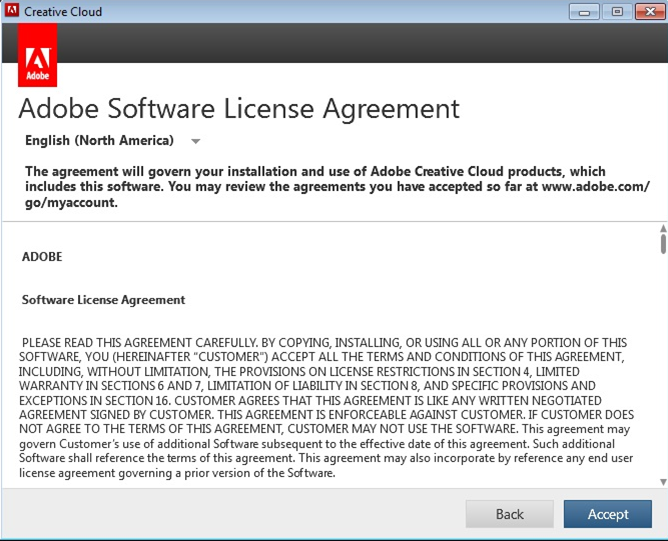
\includegraphics[width=0.7\textwidth]{adobe.png}
				\caption{Average Terms of Service Agreement\footnotemark}
			\end{figure}
		\end{column}
	\end{columns}

	\footnotetext{that you never read}
\end{frame}

\begin{frame}{Privacy}
	Since all free software is required to publish its source code, you or
	anyone else and read it to spot any potential privacy breaching code.

	\pause

You can see exactly what is executed on your CPU and make an informed decision
	to run it or not!
\end{frame}

\begin{frame}{Business}
	\begin{columns}
		\begin{column}{0.5\textwidth}
			Most modern companies rely on open source software to
			build their products.
			\begin{itemize}
				\item Discord: \url{https://discord.com/licenses}
				\item Redhat: Accquired by IBM for \$30 Billion
				\item Meta: \url{https://opensource.fb.com/}
				\item Google: Kubernetes
			\end{itemize}
		\end{column}
		\begin{column}{0.5\textwidth}
			\begin{figure}
				\centering
				
\includegraphics[width=0.7\textwidth]{redhat.jpg}
				\caption{Red Hat Enterprise Linux logo}
			\end{figure}
		\end{column}
	\end{columns}
\end{frame}

\begin{frame}{Closing Remarks}
	\begin{center}
		\Huge Thank you!
	\end{center}
\end{frame}

\begin{frame}{Closing Remarks}
	\begin{columns}
		\begin{column}{0.5\textwidth}
			\textbf{Officers}
			\begin{figure}
				\centering
				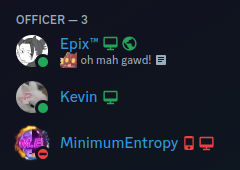
\includegraphics[width=0.60\textwidth]{officers.png}
			\end{figure}
		\end{column}
		\begin{column}{0.5\textwidth}
			The information in this presentation will be made
			available\footnotemark on our website!\\
			\url{https://lug.cs.uic.edu}
			
			\bigskip
			Join our Discord!

			\begin{figure}
				\centering
				\includesvg[width=0.5\textwidth]{lug-discord.svg}
				\caption{\url{https://discord.gg/NgxTR7PX5e}}
			\end{figure}
		\end{column}
	\end{columns}

	\footnotetext{sooner or later}
\end{frame}

\end{document}

% vim: set tw=80 ts=4 sw
